\documentclass[10pt]{beamer}
\usepackage{inputenc}
\usepackage{graphicx}
\usepackage{enumerate}
\usepackage{listings}
\usepackage{caption}
\captionsetup{font=scriptsize,labelfont=scriptsize}
\usepackage{amsmath}
\usepackage{amssymb}
\usepackage{amsthm}
\usetheme{metropolis}    
\usepackage{hyperref}
\usepackage{verbatim}
\usepackage{alltt}
\usepackage{xcolor}
\usepackage{appendixnumberbeamer}
\usepackage{subcaption}
\usepackage{animate}
\usepackage{xmpmulti}
\usepackage{threeparttable}
\usepackage{booktabs}
\usepackage{setspace}


\def\signed #1{{\leavevmode\unskip\nobreak\hfil\penalty50\hskip1em
		\hbox{}\nobreak\hfill #1%
		\parfillskip=0pt \finalhyphendemerits=0 \endgraf}}

\newsavebox\mybox
\newenvironment{aquote}[1]
{\savebox\mybox{#1}\begin{quote}\openautoquote\hspace*{-.7ex}}
	{\unskip\closeautoquote\vspace*{1mm}\signed{\usebox\mybox}\end{quote}}
\newcommand{\backupbegin}{
	\newcounter{finalframe}
	\setcounter{finalframe}{\value{framenumber}}
}
\newcommand{\backupend}{
	\setcounter{framenumber}{\value{finalframe}}
}
\usepackage[normalem]{ulem}
\useunder{\uline}{\ul}{}
\makeatletter
\setbeamertemplate{footline}
{
	\leavevmode%
	\hbox{%
		\begin{beamercolorbox}[wd=.15\paperwidth,ht=2.25ex,dp=1ex,center]{institute in head/foot}%
			\usebeamerfont{title in head/foot}%
			%  \insertshortauthor 
		\end{beamercolorbox}%
		\begin{beamercolorbox}[wd=.6\paperwidth,ht=2.25ex,dp=1ex,center]{institute in head/foot}%
			\usebeamerfont{title in head/foot}%
			\insertshorttitle
		\end{beamercolorbox}%
		\begin{beamercolorbox}[wd=.15\paperwidth,ht=2.25ex,dp=1ex,center]{institute in head/foot}%
			\usebeamerfont{title in head/foot}%
			\insertshortdate
		\end{beamercolorbox}%
		\begin{beamercolorbox}[wd=.1\paperwidth,ht=2.25ex,dp=1ex,right]{institute in head/foot}%
			\usebeamerfont{title in head/foot} 
			\insertframenumber{} / \inserttotalframenumber\hspace*{2ex} 
	\end{beamercolorbox}}%
}

\definecolor{blueucl}{RGB}{0,87,156} 
\setbeamercolor{itemize item}{fg = blueucl}
\setbeamercolor{itemize subitem}{fg = blueucl}
\setbeamercolor{enumerate item}{fg = blueucl}
\setbeamercolor{enumerate subitem}{fg = blueucl}
\setbeamertemplate{itemize item}[triangle]
\setbeamercolor{progress bar}{fg=blueucl}
\setbeamercolor{alerted text}{fg = blueucl}

\lstset{numbers=left, numberstyle=\tiny, stepnumber=1,firstnumber=1,
	numbersep=5pt,
	stringstyle=\ttfamily,
	basicstyle=\footnotesize, 
	showstringspaces=false, 
	stringstyle=\color{blueucl}, 
	tabsize=1
}
\makeatother
\setbeamertemplate{caption}[numbered]
\newcommand{\ep}{\varepsilon}
\newtheorem{assumption}{Assumption}
\newtheorem{proposition}{Proposition}

\title[Flow Trading]{Testing Flow Trading Format \\in the Laboratory}
\author[YL]{Dan Friedman, Yilin Li, Kristian L\'opez Vargas}
\institute[UCSC]{University of California, Santa Cruz}  
\date[June 2023]{June 7th, 2023}

\begin{document}
\maketitle

\begin{frame}{Summary}
    \begin{itemize}
        \item \textbf{Broad Motivation}: \textbf{What is a good design for financial market} in the presence of \textbf{costly} processing and communication \textbf{technology} and HFTs?
        \item \textbf{Design flaws} in markets, the laws of physics and heterogeneity in access to technology create  an unfair playing field
        \item Outcomes: social \textbf{inefficiencies} and substantial \textbf{inequality}
        \item We study a design that aims to correct the flaws: the \textbf{Flow Market (FLOW, hereafter, Kyle \& Lee, 2017)}
        \item We conduct \textbf{laboratory study} comparing the \textbf{FLOW} format with the established \textbf{CDA} format
        \item We want to study the \textbf{convergence} to the underlying competitive equilibrium (CE) price, \textbf{efficiency}, \textbf{price dispersion}, message intensity and inequality, etc. 
    \end{itemize}
\end{frame}

\begin{frame}{Motivation}
    \begin{itemize}
        \item Exchanges based in CDA exhibit several important \textbf{flaws}.
        \item \textbf{CDA} forces \textbf{discreteness} in price and quantity (demand and supply curves are discontinuous step functions). 
    \end{itemize}
    \textbf{Problem 1: Price Impact} 
    \begin{itemize}
        \item CDA only allows agents to submit intentions to \textbf{trade at once} (e.g. BUY, 100 Shares, at \$20)
        \item Theory and vast evidence show that if processing/sending orders is cheap, traders' optimal strategy is to \textbf{shred} orders not to have a \textbf{price impact} (send many orders with small quantities to obtain a good average price)
        \item Since the \textbf{access} to computation and communication technology is \textbf{heretogeneous}, CDA effectively favors a subset of agents
        \item The flow format moves the implementation of \textbf{shredding into the exchange}, leveling the field
    \end{itemize}
\end{frame}

\begin{frame}{Motivation}
    \textbf{Problem 2: Picking Off} 
    \begin{itemize}
        \item The CDA rewards traders with high speed and short-term information. How?
        \item Excess demand or supply occur often at the trading price, making the rationing rule relevant. The rule is usually based on time priority, creating a comm-tech arms race among traders
        \item The outcome is a massive cooperation dilemma % BCS: better off without investing in comm-tech
        \item Who is to blame? The HFTs or the CDA built-in design flaws?
        \item We think a design fix is better than heavy handed solutions (\textbf{FLOW}, IEX, FBA, etc)
        \item Which design is better? \textbf{Observational data} is insufficient to resolve the question. \textbf{Experimentation} is necessary. 
    \end{itemize}
\end{frame}

\begin{frame}{Related Literature}
    \begin{itemize}
    % \item What is the optimal trading strategy when there is \textbf{price impact}?
    %\item Vayanos (1999) and Du and Zhou (2017) show that agents prefer to \textbf{smooth trade} across rounds to limit price impact when information about endowments is private.
    
    \item Vayanos (1999), Du and Zhou (2017) show that \textbf{smooth trading} is equilibrium behavior when information about endowments is private. 
    % Obiz (2017) present a similar result in a continuous-time model with many competitors. % vayanos1999strategic

    \item Kyle \& Lee (2017) and Budish et al (2015) highlight the design problem and both propose a design change. KL17 propose the ``flow'' design; and BCS15 propose the frequent batch auction (FBA). % kyle2017toward; budish2015highfrequency

    \item Aldrich and Friedman (2022) theoretically study the IEX format (speed bumps and pegged orders). % aldrich2022order

    %  \item In contrast, Rostek et al. (2015) argue that allowing for higher trading frequency increases welfare in symmetric information markets. 

    \item Budish et al (2020) discusses the existing \textbf{lack of incentives to adopt new market designs} that reduce latency arbitrage and deactivates the high-frequency trading arms race. % budish2020theory

    \item Budish et al (2022) extend the flow trading design to multiple assets. % budish2022flow

    % \item Vayanos (1999): When information about endowments is private (and independent), smooth trading constitutes an equilibrium in a multiple-round setting. Du and Zhou (2017) predicts the same outcome in a similar setting. 
    % \item In a continuous-time model, Kyle et al. Obiz (2017) show that agents trade gradually to limit price impact.
    % \item Biais, Foucault, and Moinas (2013) shows that the ability to privately acquire information leads to an overinvestment in speed. 

    %where strategics agents receive random stock endowments ( private info) and trade to share dividend risk 
    %\item Du and Zhou (2017)
    %\item Biais, Foucault, and Moinas (2013) \item Dynamic Thin Markets (2015):

\end{itemize}
\end{frame}

\begin{frame}{Related Literature}
    \begin{itemize}
        \item  Biais, Foucault, and Moinas (2015) show that the ability to privately acquire information leads to an \textbf{over-investment in communication speed}. % biais2015equilibrium
        %$\rightarrow$ Net welfare gains from removing speed-related rents. 
    
    
        % This occurs when exchange trading fees are competitive but exchages can earn profits from the sale of speed technology -> little incentives for socially optimal market design.
        \item Many studies have compared CDA to other formats under different settings (e.g., Friedman, 1996 \& 1999)
    
        \item Aldrich \& Lopez Vargas (2020) compare CDA with Frequent-Batch Auctions (FBA). % aldrich2020experiments

        %\item Andryl \& Shikilko (2016) find that exogenously reducing available trading speed diminishes adverse selection and, overall, liquidity improves significantly. 

        % \item Since only CDA is the prefered market design, laboratory settings are required to empirical compare its performance to other formats.
    
        \item ...
    \end{itemize}
\end{frame}

\begin{frame}{Market Format 1: The Continuous Double Auction (CDA)}
    \begin{itemize}
        \item Standard limit orders have \textbf{three parameters}:$\rightarrow$ ``\underline{Buy/sell} up to \underline{$Q_{max}$} (shares) at a price of \underline{$P$} (dollars per share) or better."
        \item Order submission can happen at \textbf{any moment} of time. 
        \item If one traders' order does not ``\textbf{cross the market}'', their buy/sell limit orders remains in the book. 
        \item If she does, then it transacts immediately against the best price(s) on the other side of the market.
        \item Strict \textbf{(price, time) priority}. If there is a price tie, then older orders are filled first.
    \end{itemize} 
\end{frame}

\begin{frame}{Market Format 1: The Continuous Double Auction (CDA)}
    For a \textbf{buy order} placed at time $t_0$, let $Q_{(t_{0},t)}$ denote the cumulative \textbf{quantity executed} in interval $[t_0, t ]$ for $t > t_{0}$:
    \begin{align}
    Q_{(t_{0},t)}=
    \begin{cases}
    Q_{max} & \text{ if } p_{min(t_{0},t)} < P \\
    \alpha(t_{0},t)Q_{max} & \text{ if } p_{min(t_{0},t)} = P  \\
    0  & \text{ if } p_{min(t_{0},t)} > P \\
    \end{cases}
    \end{align}
    where $\alpha(t_{0},t)\in [0,1]$ depends on the rationing rule and $p_{\min}(t_0,t)$ is defined as the minimum price $p(t)$ during the interval $t \in [t_0,t]$. \\
    \vspace{1cm}
    It is similar for the individual supply curve. It is a non-decreasing step function.
\end{frame}

\begin{frame}{Market Format 1: The CDA - Example - Individual}
    \begin{figure}
        \centering
        
\includegraphics[width=\textwidth]{figures/cda.png}
        \caption{Standard Limit Orders}
        \label{fig:cda}
    \end{figure}
\end{frame}

\begin{frame}{Market Format 1: The CDA - Example - Market}
    \begin{figure}[H]
        \centering
        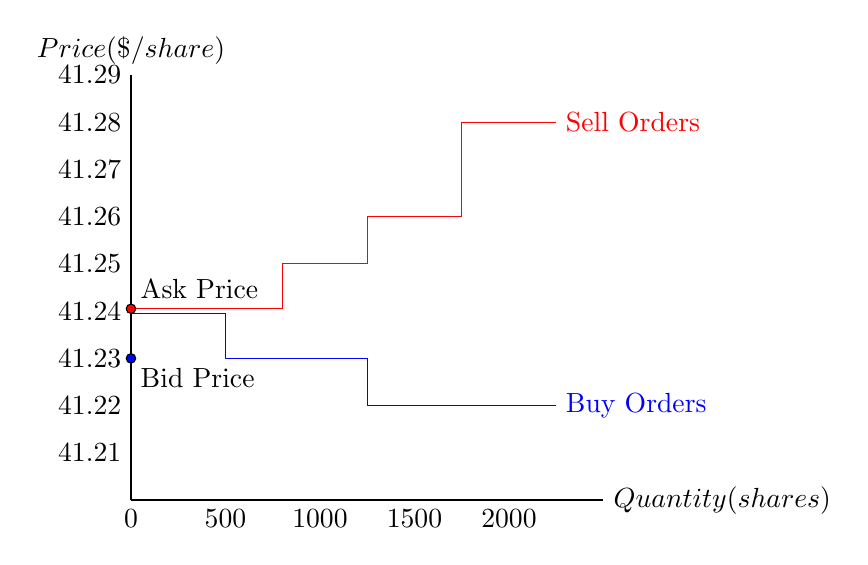
\begin{tikzpicture}[scale=.6]
        \draw[thick,-] (0,0) -- (0,9) node[above]{$Price (\$/share)$};
        \draw[thick,-] (0,0)--(10,0) node[right]{$Quantity (shares)$};
        \node[left] at (0,1) {$41.21$};
        \node[left] at (0,2) {$41.22$};
        \node[left] at (0,3) {$41.23$};
        \node[left] at (0,4) {$41.24$};
        \node[left] at (0,5) {$41.25$};
        \node[left] at (0,6) {$41.26$};
        \node[left] at (0,7) {$41.27$};
        \node[left] at (0,8) {$41.28$};
        \node[left] at (0,9) {$41.29$};
        \node[below] at (2,0) {$500$};
        \node[below] at (4,0) {$1000$};
        \node[below] at (6,0) {$1500$};
        \node[below] at (8,0) {$2000$};
        \node[below] at (0,0) {$0$};
        \draw[blue,solid] (0,3.95) -- (2,3.95) -- (2,3) -- (5,3) -- (5,2) -- (9,2) node[right]{Buy Orders} ;
        \draw[red,solid] (0,4.05) -- (3.2,4.05) -- (3.2,5) -- (5,5) -- (5,6) -- (7,6) -- (7,8) -- (9,8) node[right]{Sell Orders};
        \node[above right] at (0,4.05) {Ask Price};
        \draw[fill=red] (0,4.05) circle [radius=.1];
        \node[below right] at (0,3) {Bid Price};
        \draw[fill=blue] (0,3) circle [radius=.1];
        \end{tikzpicture}
        \caption{Standard Limit Order Book}
    \end{figure}
\end{frame}

\begin{frame}{Market Format 1: The Continuous Double Auction (CDA)}
    \begin{itemize}
        \item Since market supply and demand are discontinuous step functions of price, there is \textbf{no guarantee of a single point of intersection}: there can be excess of demand (supply), and often there is. 
        \item Hence, \textbf{an allocation rule} to determine $\alpha(t_0, t)$ is needed (time priority, or pro-rata)
        \item Often, orders are \textbf{prioritized} based on \textbf{the time they arrive}, so high speed is rewarded
        \item If an agent can \textbf{react to a relevant signal} (even if public) \textbf{faster} than other traders, she can \textbf{pick off stale orders} from other traders and reverse position after the information has spread in the market
        \item If a trader want to get a ``good" price, she need to submit several or many small orders
    \end{itemize}
\end{frame}

\begin{frame}{Market Format 2: The FLOW}
    \begin{itemize}
        \item Continuous scaled limit orders have \textbf{five parameters}: $\rightarrow$ ``\underline{Buy/Sell} up to a cumulative total of  \underline{$Q_{max}$} (shares) at maximum rate \underline{$U_{max}$} (shares per hour) at prices between \underline{$P_{L}$} and \underline{$P_{H}$} (dollars per share)."
        \item Consider a buy order, The buying rate or flow demand $U(p(t))$ is given by:
            \begin{align}
                U{(p(t))}=
                \begin{cases}
                    U_{max} & \text{ if } p{(t)} < P_{L} \\
                    (\frac{P_{H}-p(t)}{P_{H}-P_{L}})U_{max} & \text{ if } P_L \leq p{(t)} \leq P_H \\
                    0  & \text{ if } p{(t)} > P_{H} \\
                \end{cases}
            \end{align}
        where $p(t)$ is the clearing price at time $t$.
        \item Similarly, the flow supply $U(p(t))$ is also a function of $p(t)$
    \end{itemize}
\end{frame}

\begin{frame}{Market Format 2: FLOW - Example - Individual}
    \begin{figure}
        \centering
        
\includegraphics[width=\textwidth]{figures/flow.png}
        \caption{Continuous Scaled Limit Orders}
        \label{fig:flow}
    \end{figure}
\end{frame}

\begin{frame}{Market Format 2: FLOW - Example - Market}
    \begin{figure}[H]
        \centering
        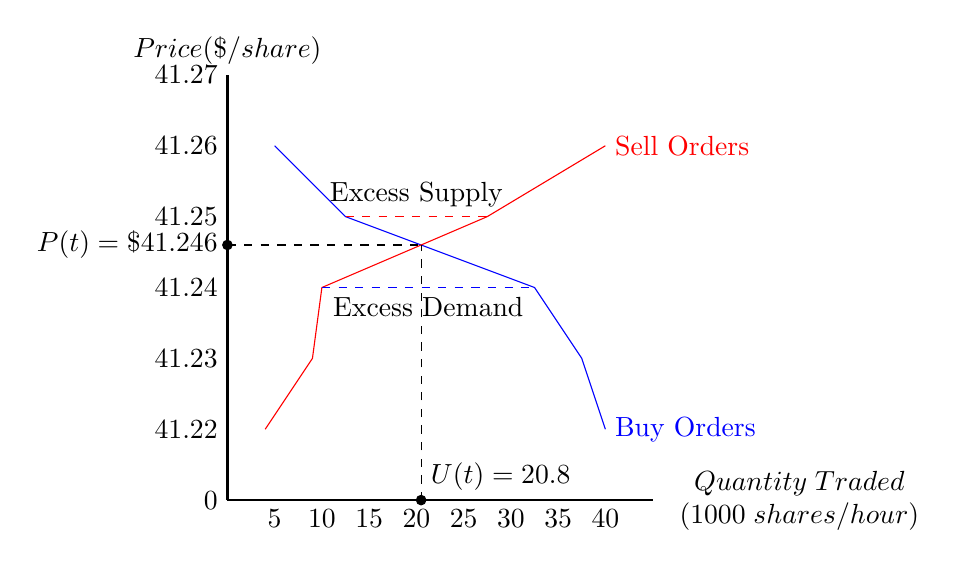
\begin{tikzpicture}[scale=0.6]
            \draw[thick,-] (0,0) -- (0,9) node[above]{$Price (\$/share)$};
            \draw[thick,-] (0,0)--(9,0) node[right]{\begin{tabular}{c}
                 $Quantity \; Traded$ \\
                 $(1000 \; shares/hour)$
            \end{tabular}};
            \node[left] at (0,1.5) {$41.22$};
            \node[left] at (0,3.0) {$41.23$};
            \node[left] at (0,4.5) {$41.24$};
            \node[left] at (0,6.0) {$41.25$};
            \node[left] at (0,7.5) {$41.26$};
            \node[left] at (0,9.0) {$41.27$};
            \node[below] at (1,0) {$5$};
            \node[below] at (2,0) {$10$};
            \node[below] at (3,0) {$15$};
            \node[below] at (4,0) {$20$};
            \node[below] at (5,0) {$25$};
            \node[below] at (6,0) {$30$};
            \node[below] at (7,0) {$35$};
            \node[below] at (8,0) {$40$};
            \node[left] at (0,0) {$0$};
            \draw[blue,solid] (1,7.5) -- (2.5,6.0) -- (6.5,4.5) -- (7.5,3) -- (8,1.5) node[right]{Buy Orders} ;
            \draw[red,solid] (0.8,1.5) -- (1.8,3) -- (2,4.5) -- (5.5,6) -- (8,7.5) node[right]{Sell Orders};
            \draw[red,dashed] (2.5,6.0) -- (5.5,6.0);
            \draw[blue,dashed] (2,4.5) -- (6.5,4.5);
            \node[black,above] at (4,6.0) {Excess Supply};
            \node[black,below] at (4.25,4.5) {Excess Demand};
            \draw[dashed] (4.1,0) -- (4.1,5.4);
            \draw[dashed] (0,5.4) -- (4.1,5.4);
            \node[above right] at (4.1,0) {$U(t)=20.8$};
            \draw[fill] (4.1,0) circle [radius=.1];
            \node[left] at (0,5.4) {$P(t)=\$41.246$};
            \draw[fill] (0,5.4) circle [radius=.1];
        \end{tikzpicture}
        \caption{Continuous Scaled Limit Order Book}
    \end{figure}
\end{frame}

\begin{frame}{Market Format 2: FLOW}
    \begin{itemize}
        \item Both the downward sloping demand schedule and upward sloping supply schedule are \textbf{piece-wise linear} functions of price $\rightarrow$ \textbf{unique} price and rate of shares per hour
        \item All continuous scaled limit orders ares treated \textbf{symmetrically} and executed \textbf{simultaneously} at the market clearing price
        \item \textbf{opportunities} to do order \textbf{shredding} are now \textbf{distributed equally} across agents, as now instructions to shred are ``moved into the exchange"
        \item Consequently, now the \textbf{fastest trader} or the ones that can send massive number of messages to update orders are not rewarded
    \end{itemize}
\end{frame}

\begin{frame}{Experiment Design: Main Elements}
    \begin{itemize}
        \item Groups of 8 traders will participate in an asset market for 22 trading periods, each lasting two minutes (2 practice + 20 payment)
        \item \textbf{Incentives to trade}: In each trading period, the computer provides a buy or sell contract committing to buy or sell up to $x$ shares at some point during the trading period (e.g., Computer will buy up to 300 shares from you at price 13 ECU at second 115)
        \item Contracts are private information
        \item Subjects' inventories are restricted to be $[-Q_{contract}, 0]$ for those with a sell contract or $[0, Q_{contract}]$ for those with a buy contract
        \item \textbf{Choice Space}: Subjects can submit or update buy and/or sell orders
        \item \textbf{Treatments}: \{CDA, FLOW\} (between-group)
        \item Three market conditions that vary in the underlying Q-P equilibrium every four periods (within-group)
    \end{itemize}
\end{frame}

\begin{frame}{Experiment Design: Interface - FLOW}
    \begin{figure}[H]
        \centering
        
\includegraphics[width=\textwidth]{figures/flow_ui.png}
        \caption{FLOW UI}
        \label{fig:flow_ui}
    \end{figure}
\end{frame}

\begin{frame}{Experiment Design: Interface - FLOW Animation}
  \animategraphics[loop,controls,width=\linewidth]{10}{figures/flow_animation/flow_animation-}{0}{419}
\end{frame}

\begin{frame}{Experiment Design: Interface - CDA}
    \begin{figure}[H]
        \centering
        
\includegraphics[width=\textwidth]{figures/cda_ui.png}
        \caption{CDA UI}
        \label{fig:cda_ui}
    \end{figure}
\end{frame}

\begin{frame}{Experiment Design: Interface - CDA Animation}
  \animategraphics[loop,controls,width=\linewidth]{10}{figures/cda_animation/cda_animation-}{0}{252}
\end{frame}


\begin{frame}{Experiment Design: Contracts}
    \begin{figure}[H]
    \centering
    \begin{subfigure}{.33\linewidth}
        \centering
        \includegraphics[scale=0.12]{production/contract/production_1.png}
        \caption{Contract Set 1 (P1 - P4 \& P17 - P20)}
    \end{subfigure}%
    \begin{subfigure}{.33\linewidth}
        \centering
        \includegraphics[scale=0.12]{production/contract/production_2.png} 
        \caption{Contract Set 2 (P5 - P8 \& P13 - P16)}
    \end{subfigure}%
    \begin{subfigure}{.33\linewidth}
        \centering
        \includegraphics[scale=0.12]{production/contract/production_3.png}
        \caption{Contract Set 3 (P9 - P12)}
    \end{subfigure}
    \caption{Contract Design}
\end{figure}
\end{frame}

\begin{frame}{Experiment Design: Procedures}
    \begin{itemize}
        \item We paid the cumulative profits of all 20 payment periods
        \item Exchange rate is 1000 ECUs = 1 USD
        \item Experiment software was designed and developed at UCSC's LEEPS Laboratory
        \item Experiment session conducted in person at LEEPS Laboratory
        \item In this presentation, we have 4 groups of FLOW and 4 groups of CDA. 
    \end{itemize}
\end{frame}

\begin{frame}{Results: Clearing Prices}
    \begin{figure}[H]
        \centering
        
\includegraphics[width=\textwidth]{figures/groups_flow_price.png}
        \caption{FLOW Price}
        \label{fig:price_flow}
    \end{figure}
    \begin{figure}[H]
        \centering
        \includegraphics[width=\textwidth]{figures/groups_cda_price_scatter.png}
        \caption{CDA Price}
        \label{fig:price_cda}
    \end{figure}
\end{frame}

\begin{frame}{Results: Flow Volume and CDA Volume}
    \begin{figure}[H]
        \centering
        
\includegraphics[width=\textwidth]{figures/groups_flow_cumsum.png}
        \caption{FLOW Volume}
        \label{fig:price_flow}
    \end{figure}
    \begin{figure}[H]
        \centering
        
\includegraphics[width=\textwidth]{figures/groups_cda_cumsum.png}
        \caption{CDA Volume}
        \label{fig:price_cda}
    \end{figure}
\end{frame}

\begin{frame}{Results: Realized Surplus}
    \begin{figure}[H]
        \centering
        
\includegraphics[width=.8\textwidth]{figures/groups_flow_surplus.png}
        \caption{FLOW Surplus}
        \label{fig:my_label}
    \end{figure}
    \begin{figure}[H]
        \centering
        
\includegraphics[width=.8\textwidth]{figures/groups_cda_surplus.png}
        \caption{CDA Surplus}
        \label{fig:my_label}
    \end{figure}
\end{frame}

\begin{frame}{Results: Filled Contracts}
    \begin{figure}[H]
        \centering
        
\includegraphics[width=.8\textwidth]{figures/groups_flow_contract.png}
        \caption{FLOW Contract}
        \label{fig:my_label}
    \end{figure}
    \begin{figure}[H]
        \centering
        
\includegraphics[width=.8\textwidth]{figures/groups_cda_contract.png}
        \caption{CDA Contract}
        \label{fig:my_label}
    \end{figure}
\end{frame}

\begin{frame}{Results: Summary Statistics}
    \begin{table}[H]
        \footnotesize
        \resizebox{\textwidth}{!}{
        \begin{threeparttable}
        \centering
            \begin{spacing}{1.25}
            \begin{tabular}{lcccc}
                \hline 
                \hline
                ~ & \multicolumn{2}{c}{$P1 - P20$} & \multicolumn{2}{c}{$P11 - P20$} \\
                ~                                & FLOW                  & CDA                  & FLOW                  & CDA      \\
                \hline
                \hline 
                 Average Price                    & 9.619                 & 8.210                & 9.470                 & 8.267    \\
                                                  & (1.427)               & (1.000)              & (1.009)               & (1.269)  \\
                 Clearing Rate (shares per second)& 9.329                 & ~                    & 9.804                 & ~        \\
                                                  & (0.380)               & ~                    & (0.169)               & ~        \\
                 Quantity Traded per Match        & ~                     & 56.474               & ~                     & 50.348   \\
                                                  & ~                     & (8.042)              & ~                     & (10.471) \\
                 $\mid$ Price - P_{CE}$\mid$      & 2.199                 & 2.097                & 1.860                 & 2.062    \\
                 Total Traded Volume (Per Period) & 932                   & 888                  & 1024                  & 885      \\
                 Realized Surplus (\%)            & 81.1                  & 85.7                 & 84.8                  & 89.9     \\
                 Market Vol./Contract Vol. (\%)   & 71.7                  & 81.4                 & 78.0                  & 83.8     \\
                 Number of Orders (Per Period)   & 28.15                 & 46.97                & 27.18                 & 47.95    \\
                 Avg. Order Size                  & 34.66                 & 19.03                & 38.55                 & 18.73    \\
                \hline
                \hline
            \end{tabular}
            \end{spacing}
            \begin{tablenotes}\noindent\justifying\scriptsize Standard deviations in parentheses. All values are averages across the four groups that participated in each market. Prices, rates and quantities ignore values of zero. \textit{Realized Surplus} is the proportion of the competitive equilibrium surplus that was obtained. \textit{Market Vol./Contract Vol.} is the proportion of the contract (infra-marginal) that was filled. \end{tablenotes}
        \end{threeparttable}}
    \end{table}
\end{frame}

\begin{frame}{Statistical Tests}
    \begin{table}[H]
        \footnotesize
        \centering
        \begin{tabular}{lcc}
            \hline 
            \hline
            (FLOW - CDA) & t-stat & p-val \\
            \hline
            Price Deviation & -0.5189 & 0.6053 \\
            Realized Surplus & -3.1493 & 0.0023 \\
            Filled Contract (\%) & -2.6158 & 0.0107 \\
            Total Traded Volume & 3.2915 & 0.0015 \\
            Order Number & -19.5391 & .0000 \\
            Order Size & 14.9954 & .0000 \\
            \hline
            \hline
        \end{tabular}
        \caption{Statistical Tests for Means (group-period level) }
        \label{tab:stat_tests}
    \end{table}
\end{frame}


\begin{frame}{Conclusions (Preliminary)}
    \begin{itemize}
    %\item No evidence of higher information efficiency 
    \item Price efficiency is similar across the two formats.
    \item Evidence of learning over time in FLOW markets. Not so much in CDA markets.
    \item After learning, FLOW markets do not show better price convergence, but do show some improvement, coming for higher rates of trading.
    \item Elements to be incorporated in experiment: heterogeneous messaging costs, costly reduction of latency, direct format competition. Other elements?
    \item Feedback is much appreciated.
    \end{itemize} 
\end{frame}



\end{document}